\documentclass[conference]{IEEEtran}
\IEEEoverridecommandlockouts
% The preceding line is only needed to identify funding in the first footnote. If that is unneeded, please comment it out.
\usepackage{cite}
\usepackage{amsmath}
\usepackage{amsmath,amssymb,amsfonts}
\usepackage{algorithmic}
\usepackage{graphicx}
\usepackage{textcomp}
\usepackage{xcolor}
\usepackage{hyperref}
\DeclareUnicodeCharacter{2212}{-}

\usepackage{background}
\usetikzlibrary{calc}

\SetBgScale{1}
\SetBgAngle{0}
\SetBgColor{black}
\SetBgContents{

\begin{tikzpicture}[overlay,remember picture]
    \draw [line width=1pt,rounded corners=5pt,]
        ($ (current page.north west) + (1cm,-1cm) $)
        rectangle
        ($ (current page.south east) + (-1cm,1cm) $);
\end{tikzpicture}}

\def\BibTeX{{\rm B\kern-.05em{\sc i\kern-.025em b}\kern-.08em
    T\kern-.1667em\lower.7ex\hbox{E}\kern-.125emX}}
    
\begin{document}

\title{CS362 (AI) InverseAI Lab Report\\
{{\footnotesize \textsuperscript{}\textbf{\href{}{}}}}
}


\author{
\IEEEauthorblockN{Jimit Patel\textsuperscript{} }
\IEEEauthorblockA{
\textsuperscript{}202051137@iiitvadodara.ac.in}
\IEEEauthorblockN{Umang Rathod \textsuperscript{}}
\IEEEauthorblockA{
\textsuperscript{}202051154@iiitvadodara.ac.in}
\and
\IEEEauthorblockN{Ritik Patidar\textsuperscript{}}
\IEEEauthorblockA{
\textsuperscript{}202051159@iiitvadodara.ac.in}
\IEEEauthorblockN{Shrut Pansuriya\textsuperscript{}}
\IEEEauthorblockA{
\textsuperscript{}202051176@iiitvadodara.ac.in}
}
\maketitle



\section*{Contents}
\section*{\textbf{Introduction}}
\section*{\textbf{Lab Assignment 1}}
\section*{\textbf{Lab Assignment 3}}
\section*{\textbf{Lab Assignment 5}}
\section*{\textbf{Lab Assignment 6}}
\section*{\textbf{\href{}{}}
}






\section{Introduction}
In these report we have included the observation,result and conclusion of the 4 experiments given to us in the lab.The 4 experiments we have included are:
\begin{enumerate}
    \item  Lab Assignment 1: Graph Search Agent for 8-Puzzle
    \item  Lab Assignment 3: TSP using Simulated Annealing
\end{enumerate}
We have understood and visualised our result in the form of tables and charts and thus discussed the same in these section.
\\
\\
We have executed the codes in Jupyter Notebook for Python.In these section we have discussed the approach to the problem.
\\
\textbf{\href{}{}}


\section{Week I Lab assignment 1 }
\textbf{Learning Objective:}
To design a graph search agent and understand the use of a hash table, queue in state space search. In this lab, we need prior knowledge of the types of agents
involved and use this knowledge to solve a puzzle called 8-puzzle.
\begin{figure}[htbp]
\centerline{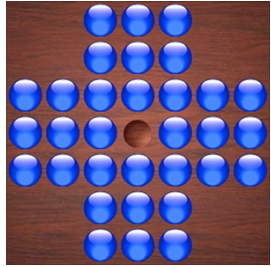
\includegraphics[width=5cm, height=4cm]{puzz.png}}
\caption{Initial and Final state of 8-Puzzle \cite}
\label{fig}
\end{figure}
8-Puzzle consist of a 3x3 matrix with the tiles numbered as shown and there is one white space available in which the tile can move.
\subsection{Part A}
Write a pseudocode for a graph search agent. Represent
the agent in the form of a flow chart. Clearly mention all the
implementation details with reasons.
\begin{figure}[htbp]
\centerline{\includegraphics[scale=0.5]{}}
\caption{}
\label{fig}
\end{figure}
\newline
\textbf{Algorithm:}
\begin{figure}[htbp]
\centerline{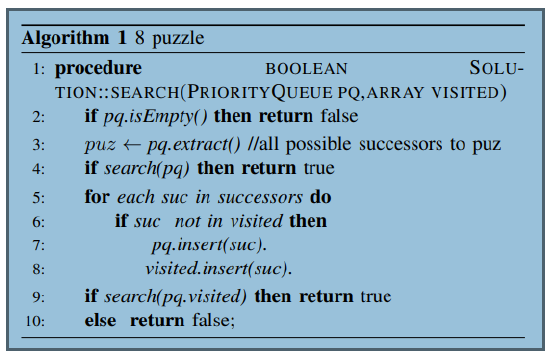
\includegraphics[scale=0.7]{alg.png}}
\end{figure}


\subsection{Part B}
Write a collection of functions imitating the environment
for Puzzle-8. Our code consists of following functions:
\begin{itemize}
    \item \textbf{Heuritic 1:} 
Heuristic for calculating the distance of goal state
using Manhattan distance.\cite{b6}
\\
\\
Parameters:
\\
current state(np.ndarray): A 3x3 array with each
cell containing unique elements as in current state
\\
goal state(np.ndarray): A 3x3 array with each
cell containing unique elements as in goal state
\\
\\
returns:
\\
heuristic1(int): Heuristic value
\\
    \item \textbf{Heuristic 2:}
Heuristic for calculating the distance of goal state
using number of misplaced tiles
\\
\\
Parameters:
\\
current state(np.ndarray): A 3x3 array with each
cell containing unique elements as in current state
\\
goal state(np.ndarray): A 3x3 array with each
cell containing unique elements as in goal state
\\
\\
returns:
\\
heuristic2(int): Heuristic value
\\
   \item \textbf{generate instance:}
\\  
\\
Parameters:
\\
goal state(np.ndarray): A 3x3 array with each cell containing unique elements representing the goal
\\
depthstate(int): The depth at which the state is to be
generated
\\
debug(bool): Get intermediate states and the heuristic
values.Default value is False
\\
\\
returns:
\\
curr state(np.ndarray): A 3x3 array with each cell containing unique elements representing the state at the given depth form, the goal state   
\\
     \item \textbf{get possible next state:}
function to get the next possible state from the current state from the environment
\\
Parameters:
\\
current state(np.ndarray): A 3x3 array representing the current states
parent(string): The path taken to reach the current state
from initial Arrangement
\\
\\
returns:
\\
possible moves(list): List of possible states from current state
\\
possible paths(list): List of possible paths moves from current state
\\

Parameters:
\\
possible moves(list): List of possible states from current state
goal state(np.ndarray): A 3x3  array representing the goal state
heuristic(Integer): An integer indicating the heuristic
function to use from 1 or 2.
possible paths(list): List of possible moves from current state
\\
\\
returns:
\\
sorted possible moves(list): List of possible states from current state, sorted according to heuristic
\\
      \item \textbf{solution:}
This function returns success if the goal state is found and prints failure if no goal state is found or the programme is strucked.
\\
Parameters:
current state(np.ndarray): A 3x3 array representing the current state
goal state(np.ndarray): A 3x3 array representing the goal state
heuristic fuction(Integer): An integer indicating the heuristic
function to use.
\\
\\
\end{itemize}

\subsection{Part C}
\\
\\
\textbf{Iterative deepening depth first search (IDDFS)} Iterative Deepening search was mainly introduced to overcome the problems faced by BFS and DFS algorithms.We do a DFS search in BFS algorithm.The graph/tree is searched in DFS pattern but is allowed to go to a certain depth only.So we do a DFS in BFS algorithm.It is an approach which takes lower space and  optimal time compared to DFS or BFS.This would be clearly explained from the following figure\cite{b1}
\begin{figure}[htbp]
\centerline{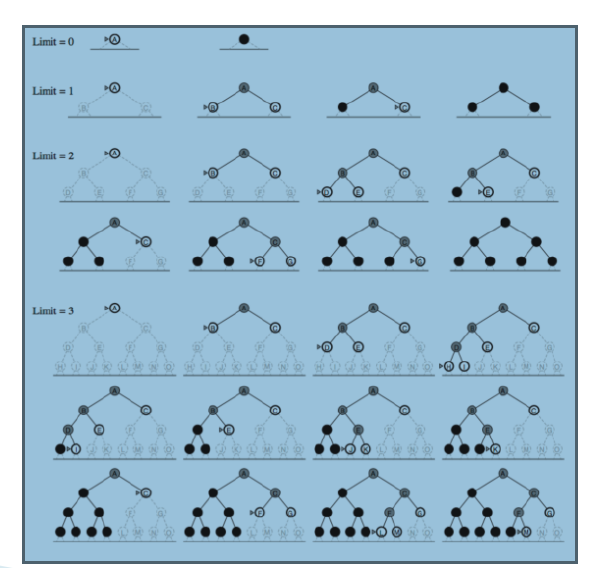
\includegraphics[scale=0.7]{itr.png}}
\caption{Iterative deepening search example\cite{}}
\label{fig}
\end{figure}
Suppose b is the branching factor and depth is d then we have time complexity ans Space Complexity as
\\
\textbf{Time Complexity:} O(b\textsuperscript{d})
\\
\textbf{Space Complexity:} O(bd)
\\
\subsection{Part D}
Considering the cost associated with every move to be the
same (uniform cost), so backtrack
and produce the path taken to reach the goal state from the
source/initial state.
\\
\\
The Code Snippet for the function is given Under as follows:
\begin{figure}[htbp]
\centerline{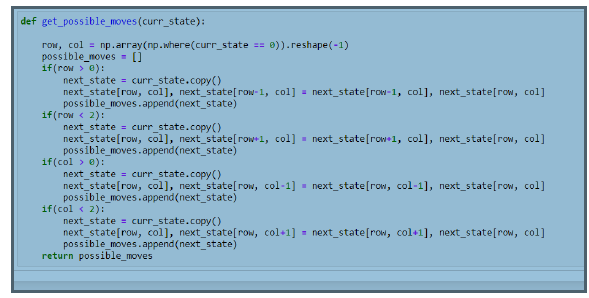
\includegraphics[scale=0.7]{fun.png}}
\caption{Function to backtrack}
\label{fig}
\end{figure}

\subsection{Part E}
\newline
Generate Puzzle-8 instances with the goal state at depth “d”.
\\
\\
The Function generating these instances is "GeneralInstances" and the snippet of output is as follows:
\begin{figure}[htbp]
\centerline{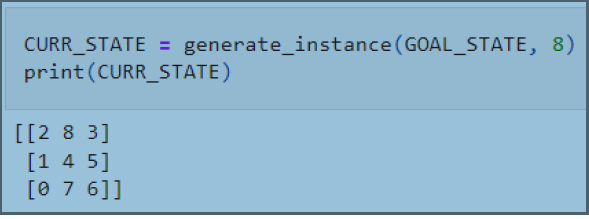
\includegraphics[scale=0.7]{bac.png}}
\caption{Function to backtrack}
\label{fig}
\end{figure}

\subsection{Part F}
\newline
Prepare a table indicating the memory and time requirements to solve Puzzle-8 instances (depth “d”) using your graph search agent.
\\
For tracking the time and memory there are packages available in python and we have used memory\_profile.The three tables generated are given below and they are made considering the 2 different hueristic function and without any hueristic function.

\begin{figure}
\centerline{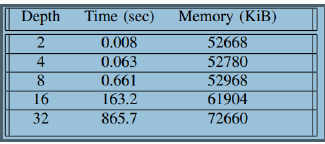
\includegraphics[scale=0.8]{usi.png}}
{        Using Manhattan Distance Heuristic}

\end{figure}
\\

\begin{figure}
\centerline{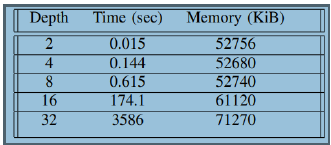
\includegraphics[scale=0.8]{mis.png}}
{        Using Misplaced tiles Heuristic}

\end{figure}
\\

\begin{figure}
\centerline{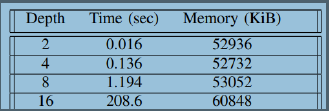
\includegraphics[scale=0.5]{wit.png}}
{        Without using any Heuristic}

\end{figure}


\section{Week 3 Lab Assignment 3}
\textbf{Learning Objective:} 
Non-deterministic Search | Simulated
Annealing For problems with large search spaces, randomized search becomes a meaningful option given partial/full-information about the domain.
\\
\\
\textbf{Problem Statement:}
Travelling Salesman Problem (TSP) is a hard problem, and is simple to state. Given a graph in which the nodes are locations of cities, and edges are labelled with the cost of travelling between cities, find a cycle containing each city exactly once, such that the total cost of the tour is as low as possible.
\\
\\
The entire code for week 3 has been coded in Jupyter notebook and you can find the link for that code here.
\href{}{}
\\
\\
Here we are visiting 25 random nodes/points.
\\
\\
\begin{figure}[htbp]
\centerline{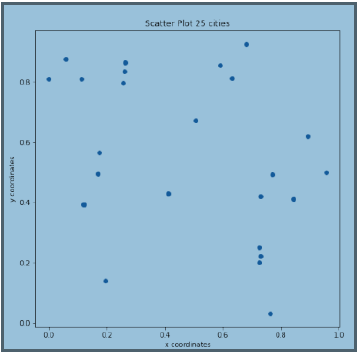
\includegraphics[scale=0.8]{ran.png}}
\caption{Scatter plot for 25 nodes}
\label{fig}
\end{figure}
\\
\\
\begin{figure}[htbp]
\centerline{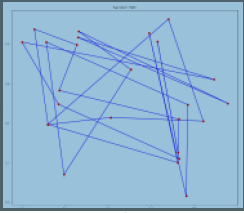
\includegraphics[scale=0.75]{sct.png}}
\caption{Comparison between the routes of 25 nodes}
\label{fig}
\end{figure}
\\
\\
\begin{figure}[htbp]
\centerline{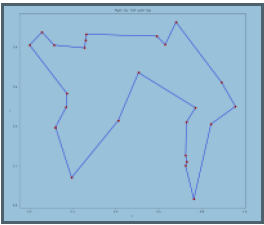
\includegraphics[scale=0.8]{apt.png}}
\caption{Fitness curve for 25 nodes}
\label{fig}
\end{figure}
\\
\\

The second plot graph in fig 7 is showing the optimal path to returning to the starting point covering all the nodes using simulated annealing to reduce the cost.
\\
\\
Fig 8 shows how simulated annealing reduces the cost over each iteration. The fitness curve shows the behavior of the cost w.r.t to the number of iterations we are running to obtain the optimal path. Initially the cost is higher than the random path cost but it significantly reduces over successive iterations and as soon as the temperature is low it becomes harder to accept the worst solution cost, there the cost moves towards optimal cost with the decrease in temperature, after some iterations the curve becomes stable - so we can conclude that not many changes are happening and the cost that we are getting is the optimal cost.





\subsection{Part A}
 For the state of Rajasthan, find out at least twenty important tourist locations.  Suppose your relatives are about to visit you next week.  Use Simulated Annealing to plan a cost effective tour of Rajasthan.  It is reasonable to assume that the cost of traveling between two locations is proportional to the distance between them.
\\
\\
We have selected 25 locations for us to visit. Now we will calculate the euclidean distance for all the pair of coordinates for all the locations. After that we will plot a random route connecting all the nodes and using simulated annealing we will find the optimal cost to cover all the locations/nodes shown in fig 10.\cite{}
\\
\\
\begin{figure}[htbp]
\centerline{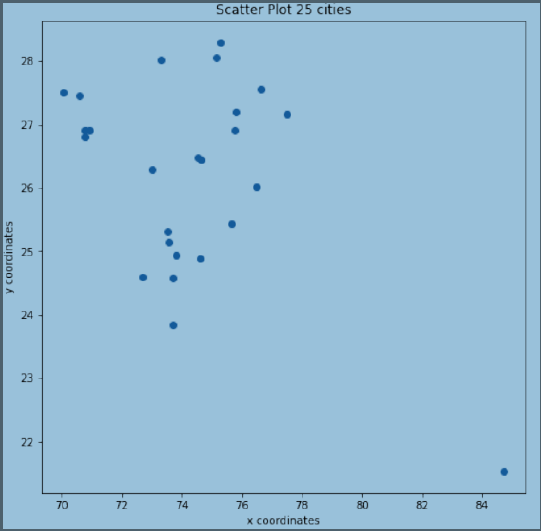
\includegraphics[scale=0.8]{sca.png}}
\caption{Scatter plot for 25 locations in Rajasthan}
\label{fig}
\end{figure}
\\
\\

\begin{figure}[htbp]
\centerline{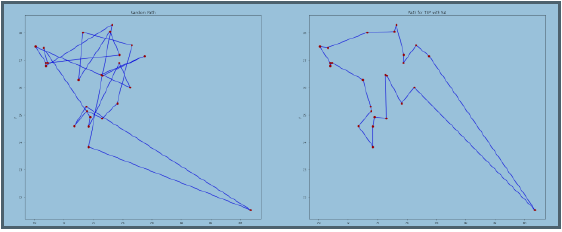
\includegraphics[scale=0.8]{opt.png}}
\caption{Optimal path for 25 locations in Rajasthan}
\label{fig}
\end{figure}
\\
\\


\subsection{Part B}
VLSI: \href{http://www.math.uwaterloo.ca/tsp/vlsi/index.html}{Dataset}
Attempt at least five problems from the above list and compare
your result
\\
\\

Here we will be doing the same procedure to find the optimal route as we did in the Rajasthan problem in the datasets from VLSI viz. 131 points, 237 points, 343 points, 379 points, and 380 points.
\\
\\
\subsubsection{XQF131 - 131 points}
\\
\\
--
\\
\\
\begin{figure}[htbp]
\centerline{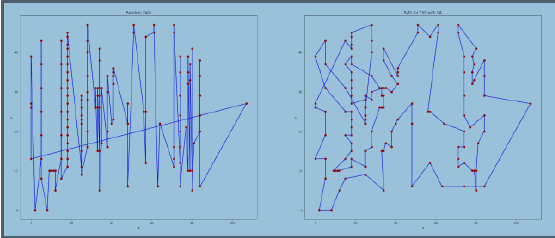
\includegraphics[scale=0.8]{gya.png}}

\label{fig}
\end{figure}
\begin{figure}[htbp]
\centerline{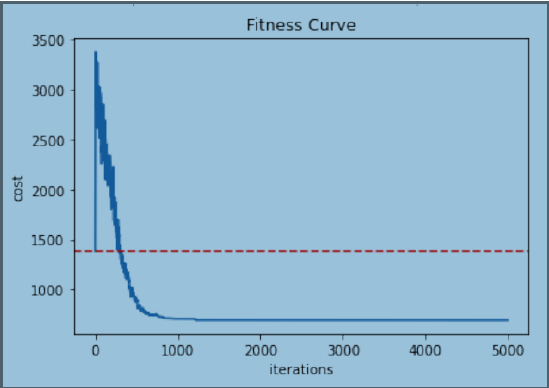
\includegraphics[scale=0.8]{plot1.png}}
\caption{Plots for 131 points}
\label{}
\end{figure}
\\
\\
\subsubsection{XQF237 - 237 points}
\\
\\
-
\\
\\
\begin{figure}[htbp]
\label{fig}
\end{figure}
\\
\\
\begin{figure}[htbp]
\caption{}
\label{fig}
\end{figure}

\subsubsection{PMA343 - 343 points}

--
\\
\\
% \begin{figure}[htbp]

% \caption{}
% \label{fig}
% \end{figure}
\\
\\
\begin{figure}[htbp]
\centerline{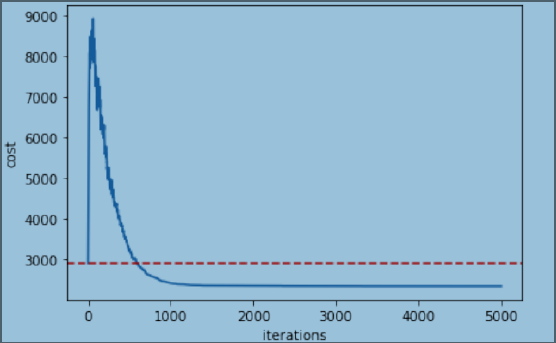
\includegraphics[scale=0.8]{abc.png}}
\caption{Plot for 379 points}
\label{fig}
\end{figure}
--
\\
\\
\begin{figure}[htbp]
\centerline{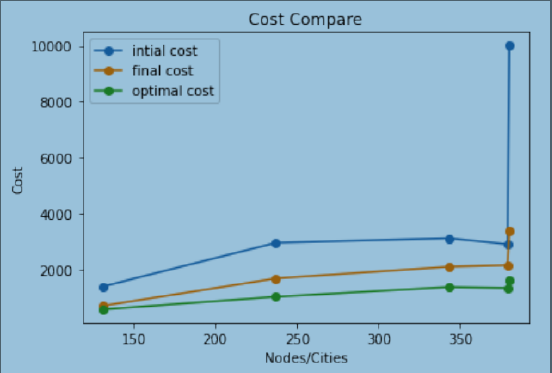
\includegraphics[scale=0.8]{bcc.png}}
\caption{Plot for 380 points}
\label{fig}
\end{figure}
\subsection{Comparing Results}
 We can see that the final cost that we are getting i.e the optimal cost is smaller than the cost that we get when we use a random route. When we compare our results with the ones given in the VLSI datasets we find that our calculated final cost is comparable with the optimal cost of VLSI.
\\
\\
% \begin{figure}[htbp]
% \caption{}
% \label{fig}
% \end{figure}
We can also further decrease the cost by increasing the iterations and using heuristic functions to solve the traveling salesman problem.
\\
\\
\begin{figure}[htbp]
\centerline{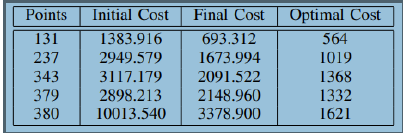
\includegraphics[scale=0.8]{mst.png}}

\label{fig}
\end{figure}

\section*{Conclusion}
\\
\\
As we have demonstrated in the above problems we have successfully solved 8 puzzle problem,Travelling salesman problem (tsp), Noughts and Crosses Game, Nim game and understood the Bayesian graphical Models to build network Graphs.
\\
\\
The importance of Heuristic plays an important role in solving the real life problems as as solving the problems in considerable amount of time as compared without Heuristic functions saving time as well as memory for big dataset problems.
\\
\\
In the Travelling Salesman problem we learned to use simulated annealing to find the optimal path or the sub optimal path.
\\
\\


\section*{Acknowledgment}
\\
We would like to thank out Prof. Pratik Shah as well TA.it is due to the lectures in AI that we were able to understand the problem as well as able to solve it.
\\
We would also like to thank the sources as well the online materials that we have used.

\begin{thebibliography}{00}
\bibitem{b1} Russell, S. and Norvig, P., 2002. Artificial intelligence: a modern approach.
\bibitem{b2}8 puzzle problem -benchpartner.com
\bibitem{b3}Shah Pratik, An Elementary Introduction to Graphical Models February
2021.
\bibitem{b6} Khemani, D., 2020. Artificial Intelligence: The Big Picture. Resonance: Journal of Science Education, 25(1).
\bibitem{b7}iddfs - stackoverflow.
\bibitem{b8}Bojan Mihaljevic,´ Bayesian networks with R November 2018.
\end{thebibliography}
\vspace{12pt}


\section{Week VII Lab Assignment VI}

\subsection{Aim}
Implemented the Expectation Maximization routine for learning parameters of a Hidden Markov Model. Used EM framework for deriving algorithms for problems with hidden or partial information.

\subsection{Hidden Markov Model}
A Hidden Markov Model (HMM) is a statistical model which is also used in machine learning. It can be used to describe the evolution of observable events that depend on internal factors, which are not directly observable.
\\
Implemented the temperature example by Hidden Markov Model and tried to implement HMM using dynamic programming.\\

% \begin{figure}[!ht]
% \centering
%     \includegraphics[scale = 0.5]{srr1.png}
%     %\caption{Fig. 1. Output of cal.cpp}
%     %\label{Fig. 1. Output of cal.cpp}
% \end{figure}\\

% Fig. 1. Output of cal.cpp

\subsection{Expectation Maximization}

The expectation maximization algorithm arises in many computational biology applications that involve probabilistic models. The expectation maximization algorithm is a refinement on this basic idea. Rather than picking the single most likely completion of the missing coin assignments on each iteration, the expectation maximization algorithm computes probabilities for each possible completion of the missing data, using the current parameters θ\^t . \\

In this process we tried to implement expectation maximization method and tried to estimate the maximum likelihood values for coins. \\



• First we take a theta as a true value or our assumption parameter. \\
• then we are iterating to find likelihood values for all coins. we use probability equation \\
   P = θ\^h ∗ θ \^( n − h ) here n = no of times coins are tossed , h is the count of heads comes and n-h will represent the number of headcounts. \\
• find normalized value and update theta with their values. \\
• Again start with the first step and perform the same operation.\\


\subsection{Observation}
In this experiment we tried to estimate the value for coins and when we perform about iteration a sufficient number of times the value of parameters coming equal to constant then we can say that we are reached at correct values of parameters. In EM-1 it shows that how values are moving toward correct values and in EM-2 they are constant now.

% \begin{figure}[!ht]
% \centering
%     \includegraphics[scale = 0.55]{srr2.png}
%     %\caption{Fig. 1. Output of cal.cpp}
%     %\label{Fig. 1. Output of cal.cpp}
% \end{figure}\\

% \begin{figure}[!ht]
% \centering
%     \includegraphics[scale = 0.6]{srr3.png}
%     %\caption{Fig. 1. Output of cal.cpp}
%     %\label{Fig. 1. Output of cal.cpp}
% \end{figure}\\

\subsection{Clustering using EM}
In this section, we tried to show clustering using EM.\\

% \begin{figure}[!ht]
% \centering
%     \includegraphics[scale = 0.6]{srr4.png}
%     %\caption{Fig. 1. Output of cal.cpp}
%     %\label{Fig. 1. Output of cal.cpp}
% \end{figure}\\


\subsection{Conclusion}
\\
We tried to implement the Hidden Markov Model and Expectation Maximization Model. Using EM we tried to find an estimation of values in coin problems and clustering of a dataset.

% \begin{figure}[!ht]
% \centering
%     \includegraphics[scale = 0.6]{srr5.png}
%     %\caption{Fig. 1. Output of cal.cpp}
%     %\label{Fig. 1. Output of cal.cpp}
% \end{figure}\\


\subsection{References}
1.) \url{http://www.cs.utoronto.ca/~strider/Denoise/Benchmark/}\\
2.) Interesting way to denoise an image using random walk: \\
\url{http://www.cs.toronto.edu/~fleet/research/Papers/BMVC_denoise.pdf}\\
3.) MRF Image Denoising: \\
\url{https://web.cs.hacettepe.edu.tr/~erkut/bil717.s12/w11a-mrf.pdf}\\
4.) Single Neuron and Hopfield Network: Chapter 40, 41, 42\\
Information Theory, Inference and Learning Algorithms, David MacKay\\
\url{http://www.inference.phy.cam.ac.uk/mackay/itila/}

%%%%%%%%%%%%%%%%%%%%%%%%%%%%%%%%%%%%%%%%%%%%%%%%%%%%%%%%%%%%%%%%%%%%%%%%%%%%%

\section{Lab Assignment 5}
 To model the low level image processing tasks in the framework of Markov Random Field and Conditional Random Field. To understand the working of Hopfield network and use it for solving some interesting combinatorial problems.


\section{Problem Statement}

\begin{enumerate}
\item Many low level vision and image processing problems are posed as minimization of energy function defined over a rectangular grid of pixels. We have seen one such problem, image segmentation, in class. The objective of image denoising is to recover an original image from a given noisy image, sometimes with missing pixels also. MRF models denoising as a probabilistic inference task. Since we are conditioning the original pixel intensities with respect to the observed noisy pixel intensities, it usually is referred to as a conditional Markov random field.  Refer to (3) above. It describes the energy function based on data and prior (smoothness). Use quadratic potentials for both singleton and pairwise potentials. Assume that there are no missing pixels. Cameraman is a standard test image for benchmarking denoising algorithms. Add varying amounts of Gaussian noise to the image for testing the MRF based denoising approach. Since the energy function is quadratic, it is possible to find the minima by simple gradient descent. If the image size is small (100x100) you may use any iterative method for solving the system of linear equations that you arrive at  by equating the gradient to zero. Extra Credit Challenge: Implement and compare MRF denoising with Stochastic denoising (reference 2).


\item For the sample code hopfield.m supplied in the lab-work folder, find out the amount of error (in bits) tolerable for each of the stored patterns.


\item Solve a TSP (traveling salesman problem) of 10 cities with a Hopfield network.  How many weights do you need for the network?  


\end{enumerate}

\section{Explanation}
\subsection{Problem 1}

This is a 512x512 grayscale image. We normalize the pixel
values to be between 0 and 1, by dividing all values by 255, and then ’binarizing’ it for the Markov Random Field by converting all the normalized pixel values below 0.5 to 0 and the rest to 1
Markov random fields sue a quadratic potential function to measure the energy potential of the image when changing a particular pixel, with respect to the neighbouring pixels.
The quadratic potential function is given by:
\begin{equation}
    E(U)= \Sigma_{n=1}^{N}(u_n-v_n)^2+ \lambda \Sigma_{n=1}^{N-1}(u_n_+_1 - u_n)^2 
\end{equation}
where v is the smooth ID signal, u is the IID and E is the energy function. We ran the algorithm for 5*512*512 = 1310720 iterations.
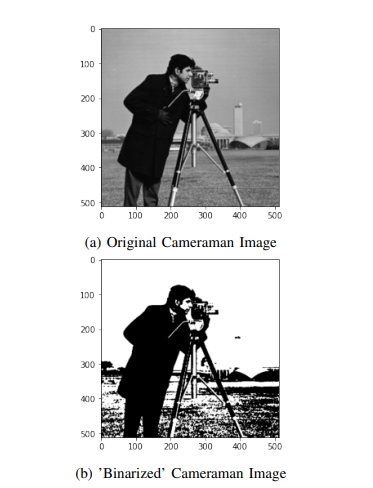
\includegraphics{Screenshot 2023-02-25 142025.png}
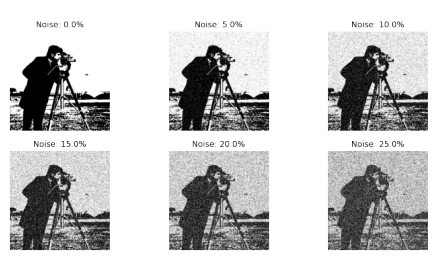
\includegraphics{Screenshot 2023-02-25 142052.png}
\subsection{Problem 2}
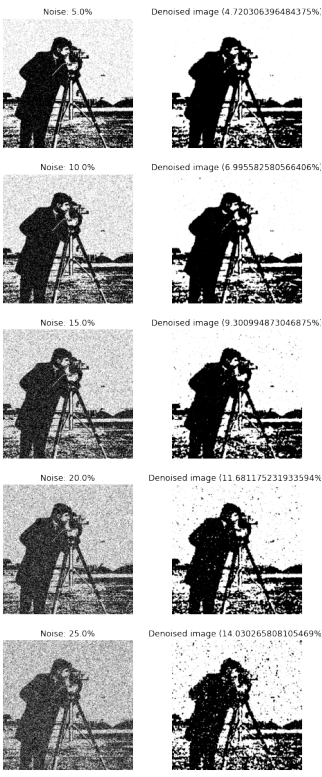
\includegraphics{Screenshot 2023-02-25 142547.png}\\
For this task, we converted the hopfield.m MATLAB codes
to Python so that we could do it in the same Notebook as the other parts. The network was trained using Hebb’s rule, as in the file and then they were noised by changing some random pixel values. At max, 15 pixel values were noised. We can see that suprisingly, the network can correct up to max 8 errors.
\subsection{Problem 3}

\includegraphics{Screenshot 2023-02-25 143219.png}
This is the usual famous NP-hard problem of Travelling
Salesman, that is done using the Hopfield Networks.
Since in a Hopfield Network, each node is connected to
the other node, we needed a total of 10x10 = 100 weights.
We first generate 10 cities randomly. And then let the hopfield network predict an optimal least
path cost.
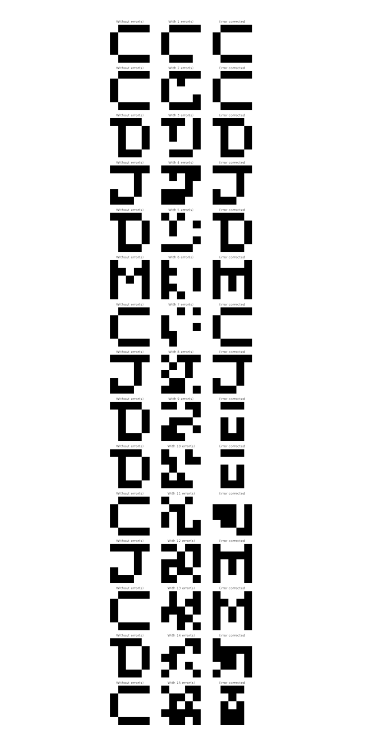
\includegraphics{Screenshot 2023-02-25 143543.png}
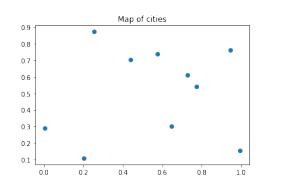
\includegraphics{Screenshot 2023-02-25 143726.png}

% \section{GITHUB LINK}
% Click {\color{blue}\href{https://github.com/Sparsh1000/AI-Lab-Report-/tree/main/lab6}{here}} to visit the Lab7 GitHub repository.

\section{References}
\begin{enumerate}
    \item  \href{http://www.cs.utoronto.ca/~strider/Denoise/Benchmark/}{http://www.cs.utoronto.ca/~strider/Denoise/Benchmark/}
    \item  Interesting way to denoise an image using random walk: \href{http://www.cs.toronto.edu/~fleet/research/Papers/BMVC_denoise.pdf} {http://www.cs.toronto.edu/~fleet/research/Papers/
    BMVC_denoise.pdf}
    \item MRF Image Denoising: \href{https://web.cs.hacettepe.edu.tr/~erkut/bil717.s12/w11a-mrf.pdf}
{https://web.cs.hacettepe.edu.tr/~erkut/bil717.s12/w11a-mrf.pdf }
    \item Single Neuron and Hopfield Network: Chapter 40, 41, 42 Information Theory, Inference and Learning Algorithms, David MacKay
\href{http://www.inference.phy.cam.ac.uk/mackay/itila/}
{http://www.inference.phy.cam.ac.uk/mackay/itila/}

\end{enumerate}

\end{document}

